%
%  progress-presentation.tex
%  src
%
%  Created by Illya Starikov on 09/16/17.
%  Copyright 2017. Illya Starikov. All rights reserved.
%

% \documentclass[notes,xcolor=dvipsnames]{beamer}       % print frame + notes
% \documentclass[notes=only,xcolor=dvipsnames]{beamer}   % only notes
\documentclass[xclolor=dvipsnames]{beamer}            % only frames

\usepackage{amssymb,amsmath,verbatim,graphicx,microtype,upquote,units,booktabs,akkwidepage}

\newcommand{\chapterNumber}[1]{
    \setcounter{section}{#1}
    \addtocounter{section}{-1}
}

\title{Presentation \#1}
\subtitle{Senior Design (Comp Sci 4096)}
\author{Illya Starikov, Ian Howell, Deacon Seals, Michael Harrington, Luke Parton, Eric Michalak, Adam Evans}
\date{Sometimes In The Future}
\institute{Missouri University of Science and Technology}

\begin{document}
\begin{darkframes}
    \maketitle

    \hugeslide{Introduction}

    \begin{frame}
        \frametitle{The Game-Plan}
        \framesubtitle{For Now\ldots}
        We are delivering:

        \begin{itemize}
            \item Mobile game (iOS and Android) with server back-end
            \item Rectangular chunk of land as the board/play area
            \item Paint the land your team's color by running around
            \item Whichever team has the most area painted after a set time wins
        \end{itemize}

        \presentby{Illya Starikov}{2}
    \end{frame}


    \begin{frame}
        \frametitle{The Game-Plan}
        \framesubtitle{For The Future\ldots}

        We plan to deliver:

        \begin{itemize}
            \item End of the semester (hopefully)
            \item Have a public launch --- with monetization options
        \end{itemize}

        \presentby{Deacon Seals}{1}
    \end{frame}


    \begin{frame}
        \frametitle{Customer Related}

        \begin{description}
            \item[Inteded Beneficiary] College students (i.e., a campus club like Humans vs. Zombies)
            \item[\phantom{Placeholder---} Users]           As aforementioned.
            \item[Provides Users With] An entertaining game and a fun way to get outside and exercise.
        \end{description}

        \presentby{Luke Parton}{1}
    \end{frame}


    \begin{frame}
        \frametitle{Design}
        \framesubtitle{The Human Interaction}

        \begin{enumerate}
            \item Join a game (either ``the public game'' or custom game)
            \item When game starts, run around in physical space
            \item Tap to select and use items
        \end{enumerate}

        Along with this, there will be leaderboards, trophies, achievements, and possibly challenges.

        \presentby{Eric Michalak}{1 -- 2}
    \end{frame}


    \begin{frame}
        \frametitle{Design}
        \framesubtitle{The Human Interaction (Introduction)}

        The game will be similar to most human-based multiplayer games.

        \begin{itemize}
            \item A settings menu will allow users to customize the sound, paint transparency, and other relevant game mechanics.
            \item There are two games modes: a custom game and a public game.
                \begin{itemize}
                    \item Custom games lets a player change all parameters of the game.
                    \item Public games a pre-configured games that count towards leaderboards.
                \end{itemize}
        \end{itemize}

        Whatever can be offloaded to the client side will be done on the client side, all synchronous game data will be pushed to the server.
        \presentby{Ian Howell}{1}
    \end{frame}


    \begin{frame}
        \frametitle{Design}
        \framesubtitle{The Architecture}

        \begin{figure}[!ht]
            \centering
            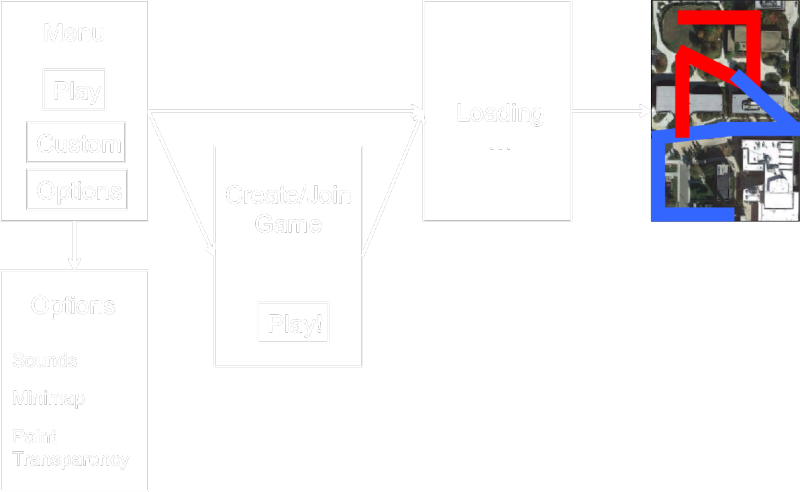
\includegraphics[width=.75\textwidth]{./assets/storyboard.png}
            \caption{The Main Storyboard}
        \end{figure}
        \presentby{Ian Howell}{0}
    \end{frame}


    \begin{frame}
        \frametitle{Lessons Learned}
        \framesubtitle{Mistakes Were Made. Lessons Were Learned.}

        What worked:

        \begin{itemize}
            \item Breaking up into server, Android, and iOS teams --- distributes workload well
            \item Swift instead of Objective-C for iOS --- safer to develop in
        \end{itemize}

        What didn't work:

        \begin{itemize}
            \item Difficult to get the map functionality we want with \syntaxbox{MKMapView} on iOS
        \end{itemize}

        \presentby{Michael Harrington \& Adam Evans}{1.5 \& 1.5}
    \end{frame}


    \begin{frame}
        \frametitle{In Closing}

        Spam Eric Michalak (Team Lead) or Illya Starikov (PR/Angel Investing) with all questions, comments, and insults.

        \begin{center}
            \begin{description}
                \item[\faComment] \href{mailto:esxmv3@mst.edu}{\nolinkurl{esxmv3@mst.edu}}
                \item[\faComment] \href{mailto:starikov@mst.edu}{\nolinkurl{starikov@mst.com}}
            \end{description}
        \end{center}

        Special thanks to the awesome team.

        \begin{center}
            \begin{description}
                \item[\faUser] Ian Howell
                \item[\faUser] Deacon Seals
                \item[\faUser] Michael Harrington
                \item[\faUser] Luke Parton
                \item[\faUser] Adam Evans
            \end{description}
        \end{center}

        \presentby{Illya Starikov}{0}
    \end{frame}

    \hugeslide{Backup Slides}

    \begin{frame}
        \frametitle{Game Model}

        \begin{figure}[!ht]
            \centering
            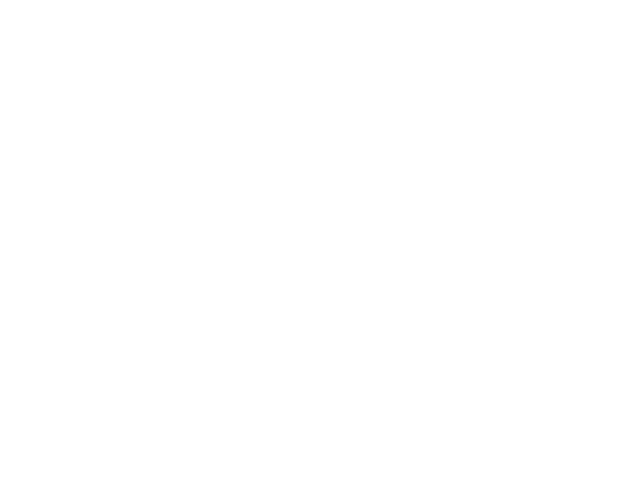
\includegraphics[width=.75\textwidth]{./assets/model.png}
            \caption{The Game Model}
        \end{figure}

    \end{frame}
\end{darkframes}
\end{document}
